\documentclass[10pt,a4paper,twocolumn]{article}
\usepackage[utf8]{inputenc}
\usepackage{amsmath}
\usepackage{amsfonts}
\usepackage{amssymb}
\usepackage{graphicx}
\usepackage{subcaption}
\author{Sven Thijssen, Emile Valcke}
\title{Inverse Reinforcement Learning}
\begin{document}
\maketitle

\section{Introduction}
Reinforcement Learning is a learning task in which an agent tries to optimize its actions, based on its state and rewards in a given environment. For Inverse Reinforcement Learning, the agent is not aware of the rewards and tries to learn the reward function by looking at an expert's behavior. Inverse reinforcement learning accomplishes two tasks: reward learning and apprenticeship learning. Reward learning is about estimating the reward function as accurately as possible, given the expert policy. Apprenticeship learning is about observing an expert and using the learned reward function to pick actions in a new environment. The main goal of this to get an optimal policy that maximizes the cumulative rewards.

\section{Literature}
Our starting point was \textit{Inverse Reinforcement Learning} by Pieter Abbeel and Andrew Y. Ng in the \textit{Encyclopedia of Machine Learning} \cite{sammut2011encyclopedia}. According to its definition, the goal of inverse reinforcement learning is to extract a reward function, given observed behavior of an agent in an environment. The main motivation for this learning task is the difficulty of defining rewards for actions performed by the agent. In this paper and all the other papers we read about Inverse Reinforcement Learning, the problem environment was modelled by the Markov Decision Process framework.\\ It is a model for a stochastic control process where the decision making is partly random and under control of a decision maker. Only the present matters, this means that previous states of an agent don't have influence on the decision making in the current state. The rules are also stationary in this world.\\\\

A finite Markov Decision Process consists of a tuple $\langle S,A,T,R \rangle$ where:

\begin{itemize}
\item $S$ is a set of states
\item $A = \{a_1,...,a_k\}$ is a set of $k$ actions
\item $T$ is a probability function $T: S \times A \times S \to [0,1]$
\item $R$ is a reward function $R: S \times A \to \mathbb{R}$
\end{itemize}

The paper \textit{“Inverse reinforcement learning algorithms and features for robot navigation in crowds: an experimental comparison} \cite{vasquez2014inverse} by D. Vasquez, B. Okal, and K. O. Arras,  gained us more insight in the concept of features. The binary representation of different ranges in the domain helped us setting up features for our concepts and applications. \\\\We also found a real world application of IRL in \textit{"An Application of Inverse Reinforcement Learning to Medical Records of Diabetes Treatment"} \cite{medicalpaper} by Hideki A., Masanori S., Shotaro A., Toshihiro K., Koiti H., Eiji A. and Takahide K. They used data of heart disease patients who may suffer from diabetes. The HA1C-level, an indicator for diabetes, was discretized in three levels: normal, medium and severe. The problem was defined as a MDP framework where states represent the diabetes-status of the patient and actions represent medical treatments by the doctor.\\\\ The reward function was based on the doctor's opinion. Bayesian IRL was used for the probability distribution of reward functions to link the appropriate reward function to the observation sequences. The reward function R can be represented as $r= (R_{normal},R_{medium},R_{severe})$ based on the level of diabetes. The solution after sampling was $r= (0.01, 0.98, 0.01)$. This may seem counterintuitive but is probably due to the fact that most patiens who participated in the data were already in the medium level from the beginning. Doctors may have the intuition to keep most of the patients in this state since it is very difficult to recover a patient from medium to normal state. Also the heterogeneity of the doctors and patients may have played a role in the computation of this reward function.

\section{Creative part}
For the creative part of this assignment, we have opted to implement the algorithm suggested by Pieter Abbeel and Andrew Y. Ng  in the paper \textit{Apprenticeship Learning by Inverse Reinforcement Learning} \cite{abbeel2004apprenticeship}. The incentive to implement an algorithm for inverse reinforcement learning was to fully comprehend the concept. As the saying goes, ``practice makes perfect''. The initial suggestion for the creative part was inverse reinforcement learning applied to Tic-Tac-Toe. However, because of its stochastic environment, this would have led us too far for the assignment. Therefore we have opted to apply inverse reinforcement learning on a grid world such that the concepts can easily be visualized and explained.

\subsection{Implementation}
In the algorithm, multiple approaches are suggested to compute the weights $w$. One such approach would be to use a quadratic programming solver where the problem is defined as follows:

$$\max\limits_{t, w} t$$\\
s.t. $$w^T \mu_E \geq w^T \mu^{(j)} + t, j= 0,...,i-1$$
$$\|w\|_2 \leq 1$$

Another approach is to use a projection method in which the feature expectations of a policy are recalculated in each iteration. From a practical standpoint, this seemed to be the best method to use. In each iteration $i$, the weights $w^{(i)}$ are updated as follows:\\
$$\bar{\mu}^{(i-1)} = \bar{\mu}^{(i-2)} + \frac
	{a^\intercal\cdot b}
	{a^\intercal\cdot a}
	\cdot
	a$$
where 
$$a = \mu^{(i-1)}-\bar{\mu}^{(i-2)}$$
and
$$b = \mu_E - \bar{\mu}^{(i-2)}$$

The weights are computed as follows:
$$w^{(i)} = \mu_E - \bar{\mu}^{(i-1)}$$


\subsection{Environment}
The environment on which we tested our implementation is the bicycle storage next to the Computer Science building from KU Leuven. Based on an aerial image from Google Maps (Figure \ref{fig:google}), we created a grid world environment (Figure \ref{fig:gridworld}). For each cell, we defined the following binary features:

\begin{table}[h]
\centering
\begin{tabular}{|l|l|l|}
	\hline
	Feature		&	Meaning		&	Representation\\\hline
	$\phi_0$		&	Ground		&	Brown\\
	$\phi_1$		&	Obstacle		&	Grey\\
	$\phi_2$		&	Water		&	Blue\\
	$\phi_3$		&	People		&	x\\
	\hline
\end{tabular}
\caption{Features for the grid world}
\end{table}

The aim is to learn a policy $\pi$, based on an expert demonstration $\zeta$ such that we can recover the rewards for the states in the grid world.

Our initial approach was different however. The idea was to guide the agent towards a goal position (marked by $G$ in Figure \ref{fig:gridworld}) by having a feature which represented the distance from that state to the goal state.
We both tested linearly decreasing distances and exponentially decreasing distances for states which are positioned further from the goal position. This tended not to work well, possibly because of the fact that it is too fine-grained.

\begin{figure}[h]
\begin{subfigure}[b]{0.5\textwidth}
	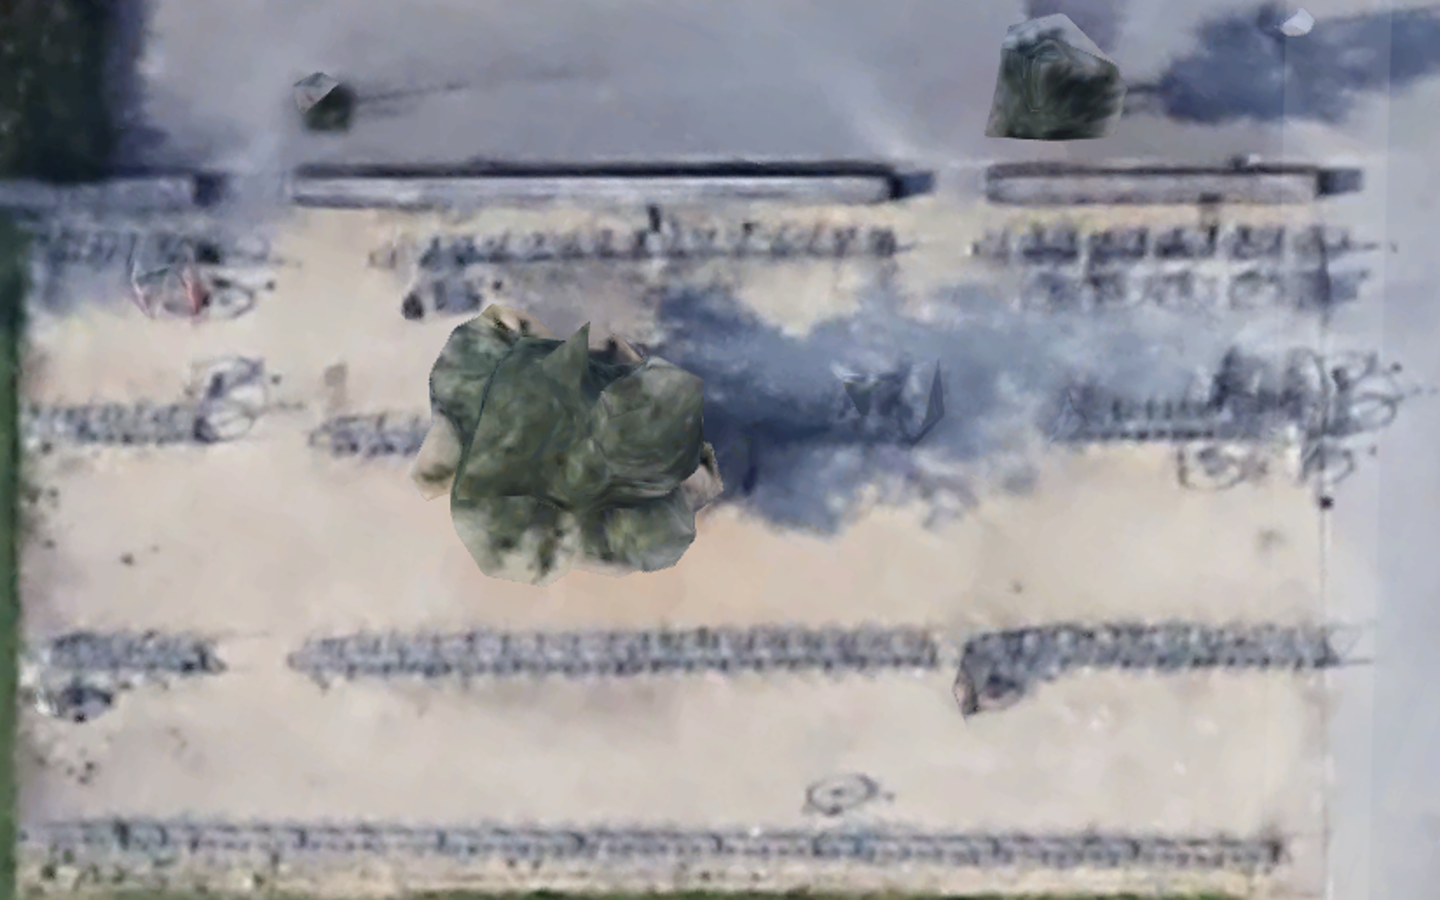
\includegraphics[width=\textwidth]{google}
	\caption{Aerial image of the environment}
	\label{fig:google}
\end{subfigure}
\begin{subfigure}[b]{0.5\textwidth}
	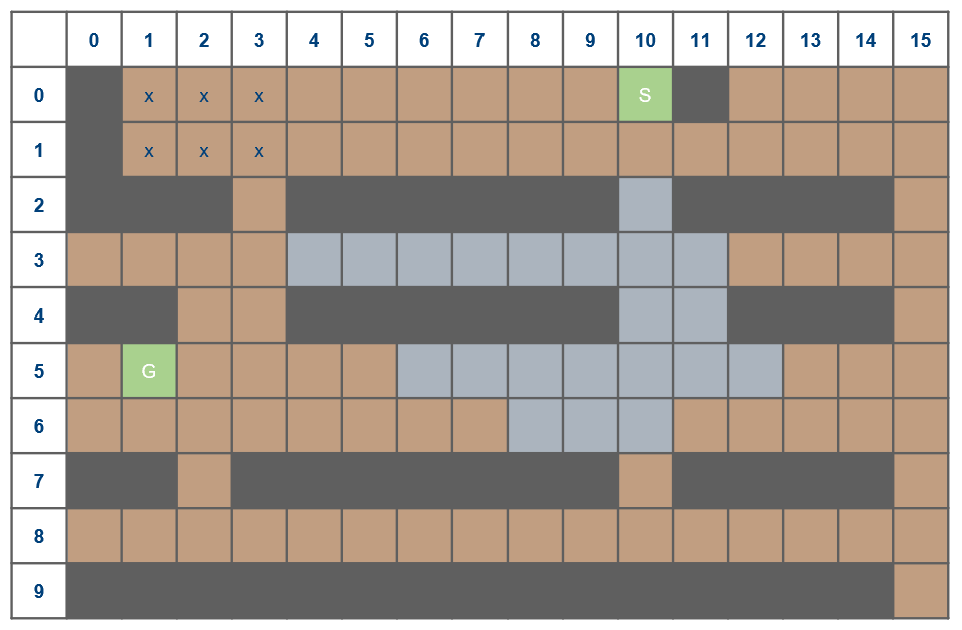
\includegraphics[width=\textwidth]{gridworld}
	\caption{Grid world of the environment}
	\label{fig:gridworld}
\end{subfigure}
\caption{Environment}
\end{figure}

\subsection{Design decisions}
For the reinforcement learning algorithm, we have chosen to implement Q-learning because of its intuitive character. The following update-rule was used since we are in a deterministic environment:
$$Q(s,a) \gets r + \gamma\cdot \max\limits_{a'}Q(s',a')$$

For the action selection mechanism, we considered two approaches: $\epsilon$-greedy and soft-max (Boltzmann). In the setting of $\epsilon$-greedy it is rather difficult to balance exploration and exploitation, whereas Boltzmann generates probabilities among all actions and at any given iteration, any action can be picked.
%TODO loops solution


\subsection{Experiments}
To gain insight in the solutions from the algorithm, we made plots of the error $t$ and the weights $w_i$ for the features $\phi_i$. In the first experiment (Figure \ref{fig:experiment1trajectory}), we have created an expert trajectory which tends to prefer through water (e.g. a duck). In Figure \ref{fig:experiment1heatmap} we see a heat map for the learned rewards in each state. We observe that the reward for states with people is low. This corresponds with the fact that the duck has avoids people. However, it is peculiar that the duck prefers obstacles over water. Again, the duck has never seen a state in with the wall feature. This means that the total sum of this feature over the trajectory is zero and thus, it is possible that an arbitrary weight can be given to this feature.
\begin{figure}[h]
\begin{subfigure}[b]{0.5\textwidth}
	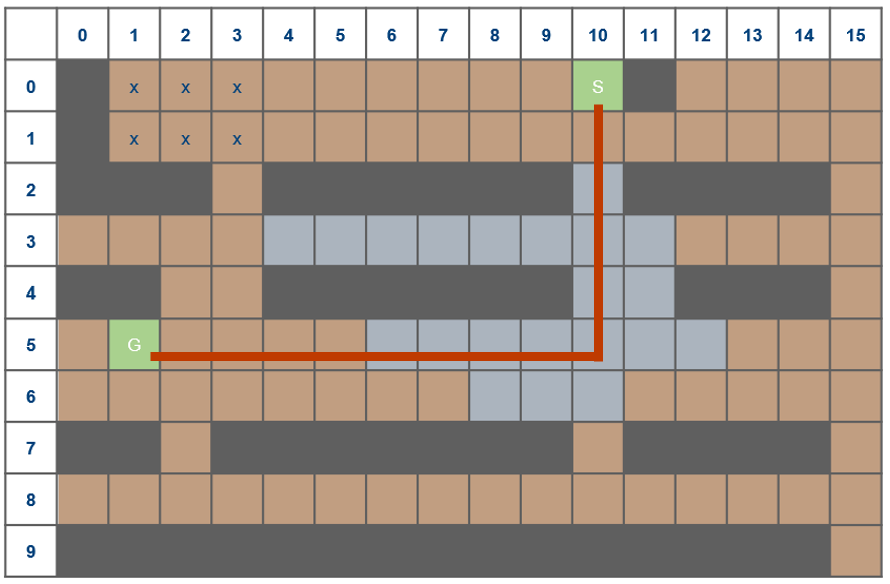
\includegraphics[width=\textwidth]{experiment_1_gridworld}
	\caption{Grid world with expert trajectory}
	\label{fig:experiment1trajectory}
\end{subfigure}
\begin{subfigure}[b]{0.5\textwidth}
	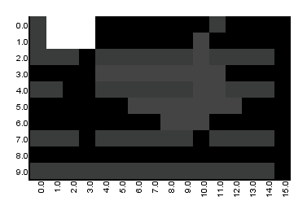
\includegraphics[width=\textwidth]{experiment_1_heatmap}
	\caption{Heat map of the rewards}
	\label{fig:experiment1heatmap}
\end{subfigure}
\caption{Experiment 1}
\end{figure}

As we can observe in Figure \ref{fig:experiment1t}, the error $t$ drops dramatically in the first iterations and then slowly converges to zero. In Figure \ref{fig:experiment1w} we see the respective values for $w$ over time. The values fluctuate around zero. This might be due to the fact that the problem is ill-posed.

\begin{figure}[h]
\begin{subfigure}[b]{0.5\textwidth}
	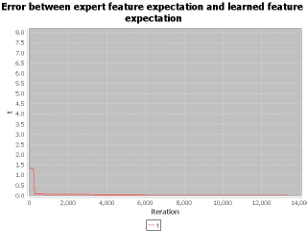
\includegraphics[width=\textwidth]{experiment_1_t}
	\caption{Error}
	\label{fig:experiment1t}
\end{subfigure}
\begin{subfigure}[b]{0.5\textwidth}
	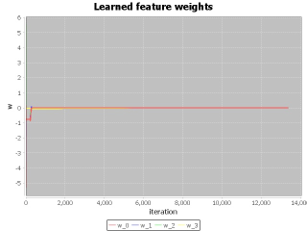
\includegraphics[width=\textwidth]{experiment_1_w}
	\caption{Weights}
	\label{fig:experiment1w}
\end{subfigure}
\caption{Experiment 1}
\end{figure}

\newpage

For a second expert trajectory (Figure \ref{fig:experiment2trajectory}), where the agent tends to prefer the features ground and people, we have set the threshold to a bigger value ($\epsilon= 0.1$) to avoid the slow convergence. In the heat map (Figure \ref{fig:experiment2heatmap}), we observe that states with water have high rewards, which does not correspond with the expert trajectory. Again, this might be due to the fact that the agent has never observed a state in which water is present.

\begin{figure}[h]
\begin{subfigure}[b]{0.5\textwidth}
	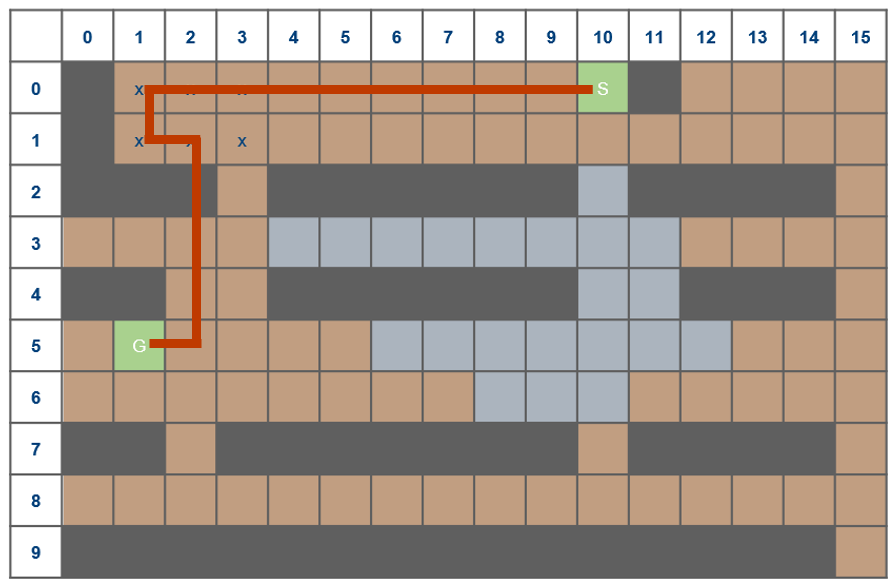
\includegraphics[width=\textwidth]{experiment_2_gridworld}
	\caption{Grid world with expert trajectory}
	\label{fig:experiment2trajectory}
\end{subfigure}
\begin{subfigure}[b]{0.5\textwidth}
	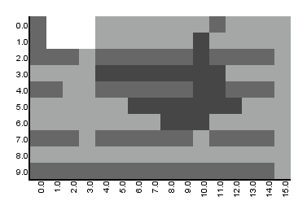
\includegraphics[width=\textwidth]{experiment_2_heatmap}
	\caption{Heat map of the rewards}
	\label{fig:experiment2heatmap}
\end{subfigure}
\caption{Experiment 2}
\end{figure}

We observe that the number of iterations has decreased drastically for a higher threshold, compared to the previous experiment. The weights in this experiment also tend to converge to zero. 

\begin{figure}[h]
\begin{subfigure}[b]{0.5\textwidth}
	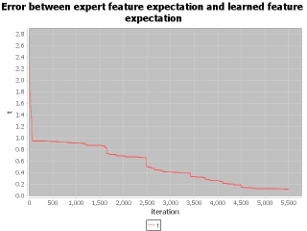
\includegraphics[width=\textwidth]{experiment_2_t}
	\caption{Error}
	\label{fig:experiment2t}
\end{subfigure}
\begin{subfigure}[b]{0.5\textwidth}
	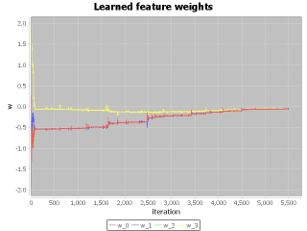
\includegraphics[width=\textwidth]{experiment_2_w}
	\caption{Weights}
	\label{fig:experiment2w}
\end{subfigure}
\caption{Experiment 2}
\end{figure}

\section{Conclusion}
When it is difficult to define a reward function in a learning task (e.g. reinforcement learning), it is possible to recover a reward function, based on demonstrations by an expert. One such approach is inverse reinforcement learning in which the rewards can be expressed in terms of the feature expectations of a policy. However, it is important to note that the optimization problem is ill-posed and the reward function can be ambiguous.

\newpage

\bibliography{references} 
\bibliographystyle{ieeetr}



\end{document}